\chapter{Singularity}
\label{chap:3}
Let us start taking analogy of robotic manipulator, Singularity is when robot looses it's degree of freedom at certain configuration or degeneration in mapping from Cartesian space to joint space. As in case when arm is at fully extended configuration when target is out of reach or at folded state when two joint axis are alined referred as internal or external singularity. When rank of mapping matrix which maps joint space to Cartesian space is is not full rank matrix then determinant of matrix is zero making it non invertible. Velocities are very large near singular states. Similarly, for control moment gyro there exist a direction about which torque can not be produced. Singularities are classified in two categories, internal and "external. If motion of gimbal angle does not produce torque in desired direction it is called "internal singularity", it occurs within saturation boundary, unlike "external singularity" in which angular momentum reaches maximum or saturation. Coming out of some singular states can be achieved by adapting null motion control law. Null motion control is changing angular momentum of spacecraft without producing torque on it. Gimbal lock is situation when all components of required torques are along singular direction. It is impassable if Null motion solution does not exist at the singularity.\cite{Leve2015}

Let us recall total angular momentum of n-CMG configuration
\begin{equation*}
\mathcal{H}_{CMG} =J^{s}_{W}\sum ^{n}_{k=1} \ \Omega _{k} \ \hat{s}_{k}
\end{equation*}
and simplified torque is expressed as bellow with $\displaystyle C=J^{s}_{W} \ \mathcal{G}_{t} diag[ \Omega _{k}]$ and $\displaystyle \mathcal{G}_{t}( \delta _{k}) =[\hat{t}_{1} \ \dotsc \hat{t}_{n}]$ 

\begin{gather*}
\tau =J^{s}_{W} \ \sum ^{n}_{k=1} \Omega _{k}\dot{\delta }_{k} \ \hat{t}_{k}\\
\tau =C\dot{\delta }
\end{gather*}As long as $\displaystyle C$ is full rank matrix $\displaystyle \tau $ in any arbitrary direction can be produced. Since $\displaystyle C_{3\times n}$ is not necessarily square matrix, Gimbal rates can be obtained by taking pseudo inverse.
\begin{equation*}
\dot{\delta }_{1\times n} =C^{T}\left( CC^{T}\right)^{-1} \tau 
\end{equation*}
If rank of $\displaystyle C\neq 3$ i.e. $\displaystyle \det C=0$ then required $\displaystyle \dot{\delta }$ can not be evaluated.For n-CMG system in singular state, all $\displaystyle \hat{t}$ are co planar and torque can not be produced normal to this plane. Let $\displaystyle \hat{u}$ be the singular vector normal to plane where all $\displaystyle \hat{t}_{k}$ are co-planar. 
\begin{equation*}
\hat{u} \cdotp \hat{t}_{k} =0
\end{equation*}


\begin{figure}[!h]
    \centering
    

\tikzset{every picture/.style={line width=0.75pt}} %set default line width to 0.75pt        

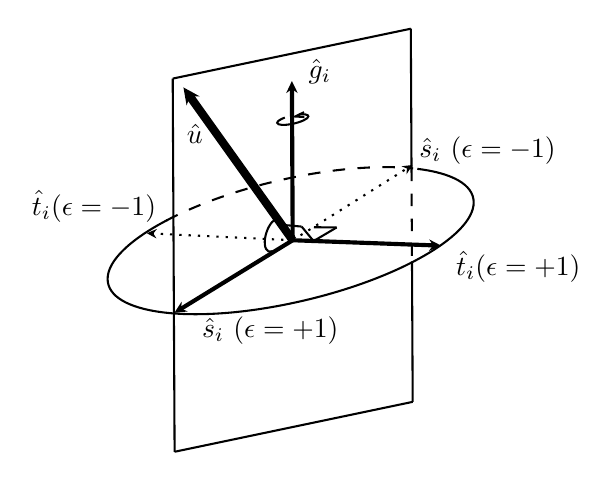
\begin{tikzpicture}[x=0.5pt,y=0.5pt,yscale=-1,xscale=1]
%uncomment if require: \path (0,348); %set diagram left start at 0, and has height of 348

%Straight Lines [id:da7916208743434348] 
\draw [line width=1.5]    (325.78,157.42) -- (243.69,207.79) ;
\draw [shift={(240.28,209.89)}, rotate = 328.47] [fill={rgb, 255:red, 0; green, 0; blue, 0 }  ][line width=0.08]  [draw opacity=0] (8.75,-4.2) -- (0,0) -- (8.75,4.2) -- (5.81,0) -- cycle    ;
%Straight Lines [id:da6063053587743079] 
\draw [line width=1.5]    (325.78,157.42) -- (429.04,161.18) ;
\draw [shift={(433.04,161.33)}, rotate = 182.09] [fill={rgb, 255:red, 0; green, 0; blue, 0 }  ][line width=0.08]  [draw opacity=0] (8.75,-4.2) -- (0,0) -- (8.75,4.2) -- (5.81,0) -- cycle    ;
%Straight Lines [id:da8584098766750565] 
\draw [line width=1.5]    (325.78,157.42) -- (325.22,46.36) ;
\draw [shift={(325.2,42.36)}, rotate = 449.71] [fill={rgb, 255:red, 0; green, 0; blue, 0 }  ][line width=0.08]  [draw opacity=0] (8.75,-4.2) -- (0,0) -- (8.75,4.2) -- (5.81,0) -- cycle    ;
%Straight Lines [id:da36750414352491156] 
\draw  [dash pattern={on 0.84pt off 2.51pt}]  (325.78,157.42) -- (409.76,104.66) ;
\draw [shift={(412.3,103.06)}, rotate = 507.86] [fill={rgb, 255:red, 0; green, 0; blue, 0 }  ][line width=0.08]  [draw opacity=0] (7.14,-3.43) -- (0,0) -- (7.14,3.43) -- (4.74,0) -- cycle    ;
%Straight Lines [id:da051548852230852926] 
\draw  [dash pattern={on 0.84pt off 2.51pt}]  (325.78,157.42) -- (223.36,152.49) ;
\draw [shift={(220.36,152.35)}, rotate = 362.75] [fill={rgb, 255:red, 0; green, 0; blue, 0 }  ][line width=0.08]  [draw opacity=0] (7.14,-3.43) -- (0,0) -- (7.14,3.43) -- (4.74,0) -- cycle    ;
%Straight Lines [id:da17659245242461763] 
\draw [line width=3]    (325.78,157.42) -- (276.96,89.13) -- (250.31,51.86) ;
\draw [shift={(246.82,46.98)}, rotate = 414.43] [fill={rgb, 255:red, 0; green, 0; blue, 0 }  ][line width=0.08]  [draw opacity=0] (11.97,-5.75) -- (0,0) -- (11.97,5.75) -- (7.95,0) -- cycle    ;
%Straight Lines [id:da48871347567863976] 
\draw    (341.17,148.01) -- (357.58,148.17) ;
%Straight Lines [id:da5947811121524507] 
\draw    (340.86,158.03) -- (357.58,148.17) ;
%Straight Lines [id:da18808003722282884] 
\draw    (318.62,146.33) -- (332.25,147.55) ;
%Straight Lines [id:da3929565984820087] 
\draw    (332.25,147.55) -- (340.86,158.03) ;
%Shape: Arc [id:dp1302171161481871] 
\draw  [draw opacity=0] (311.27,165.16) .. controls (311.04,165.28) and (310.81,165.38) .. (310.58,165.46) .. controls (306.98,166.74) and (304.84,162.5) .. (305.8,156) .. controls (306.72,149.85) and (310.07,143.88) .. (313.48,142.17) -- (312.33,153.69) -- cycle ; \draw   (311.27,165.16) .. controls (311.04,165.28) and (310.81,165.38) .. (310.58,165.46) .. controls (306.98,166.74) and (304.84,162.5) .. (305.8,156) .. controls (306.72,149.85) and (310.07,143.88) .. (313.48,142.17) ;
%Shape: Arc [id:dp4658593680079681] 
\draw  [draw opacity=0] (415.85,105.83) .. controls (440.9,108.83) and (456.52,117.16) .. (456.59,130) .. controls (456.72,155.04) and (397.59,187.75) .. (324.53,203.07) .. controls (251.47,218.39) and (192.14,210.5) .. (192.01,185.46) .. controls (191.94,172.1) and (208.74,156.56) .. (235.52,142.64) -- (324.3,157.73) -- cycle ; \draw   (415.85,105.83) .. controls (440.9,108.83) and (456.52,117.16) .. (456.59,130) .. controls (456.72,155.04) and (397.59,187.75) .. (324.53,203.07) .. controls (251.47,218.39) and (192.14,210.5) .. (192.01,185.46) .. controls (191.94,172.1) and (208.74,156.56) .. (235.52,142.64) ;
%Shape: Arc [id:dp7085048189876144] 
\draw  [draw opacity=0][dash pattern={on 4.5pt off 4.5pt}] (234.57,143.14) .. controls (258.09,130.76) and (289.52,119.63) .. (324.07,112.39) .. controls (358.2,105.23) and (389.34,103.14) .. (412.84,105.5) -- (324.3,157.73) -- cycle ; \draw  [dash pattern={on 4.5pt off 4.5pt}] (234.57,143.14) .. controls (258.09,130.76) and (289.52,119.63) .. (324.07,112.39) .. controls (358.2,105.23) and (389.34,103.14) .. (412.84,105.5) ;
%Straight Lines [id:da5865544576762574] 
\draw    (411.14,4.55) -- (411.65,105.77) ;
%Straight Lines [id:da7590207701341669] 
\draw    (239.07,40.6) -- (240.43,310.29) ;
%Straight Lines [id:da790374687044014] 
\draw    (239.07,40.6) -- (411.14,4.55) ;
%Straight Lines [id:da17494293181301823] 
\draw    (240.43,310.29) -- (412.5,274.23) ;
%Straight Lines [id:da5701402858596814] 
\draw    (411.99,172.73) -- (412.5,274.23) ;
%Straight Lines [id:da2349258321762262] 
\draw  [dash pattern={on 4.5pt off 4.5pt}]  (411.65,105.77) -- (411.99,172.73) ;
%Shape: Arc [id:dp4799622522622564] 
\draw  [draw opacity=0] (330.58,66.45) .. controls (334.42,66.13) and (337.09,66.63) .. (337.1,67.85) .. controls (337.1,69.54) and (332.07,71.96) .. (325.85,73.26) .. controls (319.63,74.57) and (314.58,74.26) .. (314.58,72.57) .. controls (314.57,71.45) and (316.78,70.01) .. (320.09,68.78) -- (325.84,70.21) -- cycle ; \draw   (330.58,66.45) .. controls (334.42,66.13) and (337.09,66.63) .. (337.1,67.85) .. controls (337.1,69.54) and (332.07,71.96) .. (325.85,73.26) .. controls (319.63,74.57) and (314.58,74.26) .. (314.58,72.57) .. controls (314.57,71.45) and (316.78,70.01) .. (320.09,68.78) ;
\draw   (333.97,64.87) -- (327.59,67.99) -- (334.21,68.38) ;

% Text Node
\draw (441.66,162.98) node [anchor=north west][inner sep=0.75pt]    {$\hat{t}_{i}( \epsilon =+1)$};
% Text Node
\draw (258,210.4) node [anchor=north west][inner sep=0.75pt]    {$\hat{s}_{i} \ ( \epsilon =+1)$};
% Text Node
\draw (415,80.4) node [anchor=north west][inner sep=0.75pt]    {$\hat{s}_{i} \ ( \epsilon =-1)$};
% Text Node
\draw (135,119.4) node [anchor=north west][inner sep=0.75pt]    {$\hat{t}_{i}( \epsilon =-1)$};
% Text Node
\draw (247,71.4) node [anchor=north west][inner sep=0.75pt]    {$\hat{u}$};
% Text Node
\draw (335,24.4) node [anchor=north west][inner sep=0.75pt]    {$\hat{g}_{i}$};
\end{tikzpicture}

    \caption{Vector representation at singular gimbal state}
    \label{fig:tikCMGSingular}
\end{figure}

From \autoref{fig:tikCMGSingular} we can see that flywheel vector $\displaystyle \hat{s}$ has either positive or negative projection on singular vector $\displaystyle \hat{u}$, hence angular momentum along singular direction is
\begin{equation*}
\mathcal{H}_{u} =\mathcal{H}_{CMG} \cdotp \hat{u}
\end{equation*}
Component of angular momentum along singular direction has constant value based on $\displaystyle \hat{u}$ that is Jacobian of $\displaystyle \mathcal{H}_{u}$with respect to $\displaystyle \delta $ is zero. Since $\displaystyle \hat{u}$ cannot lie along $\displaystyle \hat{g}$ we have $\displaystyle \hat{u} \cdotp \hat{t}_{k} =0$ for either positive or negative angular momentum component. For given $\displaystyle \hat{u}$ there are $\displaystyle 2^{n}$ singular states. Let sign of angular momentum \ component $\displaystyle \mathcal{H}_{u}$ be $\displaystyle \epsilon _{k} =sign( s\cdotp u)$ and $\displaystyle \ \hat{u} \neq \pm \hat{g}_{k}$. We have,
\begin{gather}
\hat{t}_{k} =\epsilon _{k}\frac{\ \hat{g}_{k} \times \hat{u}}{\mid \hat{g}_{k} \times \hat{u} \mid } ,\\
\hat{s}_{k} =\hat{t}_{k} \times \hat{g}_{k} =\epsilon _{k}\frac{( \ \hat{g}_{k} \times \hat{u}) \times \hat{g}_{k}}{\mid \hat{g}_{k} \times \hat{u} \mid }
\end{gather}
And angular momentum at singularity along singular direction is 
\begin{equation}
\mathcal{H}_{u} =\sum ^{n}_{k=1}\hat{s}_{k} =\sum ^{n}_{k=1} \epsilon _{k}\frac{( \ \hat{g}_{k} \times \hat{u}) \times \hat{g}_{k}}{\mid \hat{g}_{k} \times \hat{u} \mid }
\end{equation}


Projection of singular vector on total angular momentum can be evaluated for all unit singular vector $\displaystyle \hat{u} \in \mathbb{R}^{3}$ locus of all such points is singular surface and can be evaluated for given set of $\epsilon_k$. \cite{YoonSingularity}

A use full Matlab script has been developed in order to generate singular envelope of any CMG configuration with generic number of CMG units.

Results discussed here are considering Pyramid configuration of 4 CMG with skew angle $\beta =54.73^{ \circ }$ is selected for the fact that momentum distribution envelope is closed to spherical symmetry than other skew angles.\cite{ABaker2020} As we add more CMG the envelope becomes more closed to spherical but singularities singular direction increased on the order of $\displaystyle O \left( 2^{n}\right)$.

Surface plots as shown in \autoref{fig:singular_surf} are generated for each ${\displaystyle \epsilon _{k}}$ enumerating vector ${\displaystyle \hat{u}}$ as reasonable number of equidistant points on spherical surface. \autoref{fig:sing_ext} is external singular surface it is set of all singular momentum states equivalent to the maximum array angular momentum with $\epsilon =\{++++\}$ or $\epsilon =\{----\}$ we can notice there are 8 holes present, these are transition boundaries where singular vector is approaching \ towards gimbals and \ we have discontinuity at ${\displaystyle \hat{u} =\hat{g}}$. Number of circles present on external surface of skewed n-CMG configuration is ${\displaystyle 2n}$ and are present at both ends of gimbal axis initial orientation and surface associated with each $\displaystyle \epsilon $ is connected with these circles.fig:sing\_int1 is contribution of single gimbal with negative angular momentum of at least one wheel with respect to all other wheels. $\epsilon =\{-+++\}$. Notice the circular end caps similar to diverging trumpet are stretched along gimbal axis and their profile matches with holes of external surface. Internal surface has complex geometry and has both elliptical (null motion does not exist) and degenerate hyperbolic singularities (Null motion exist). Non-degenerate Hyperbolic Singularities are possible to avoid on the other hand degenerate hyperbolic singularities leads towards impassable elliptic singularity. \autoref{fig:sing_int_all} shows all internal surfaces associated with each gimbal axis, generated by permutations of $\epsilon =\{-+++\}$. \autoref{fig:sing_allOpq} is all surfaces combined together, \autoref{fig:sing_allTransp} shows another perspective of all singular surfaces of CMG pyramid. Insight from the combination of surfaces is when angular momentum of all CMG units have same sign, holes in external surface denotes singularities are present in the direction of gimbal axis and torque can not be produced in volume encapsulated by conical geometry starting from center of sphere as apex and hole being base, on the other hand if one of CMG has opposite angular momentum it can provide torque in the direction of assumed cone.

\begin{figure}
\centering
\begin{tabular}{cc}
\subcaptionbox{External Singularity\label{fig:sing_ext}}{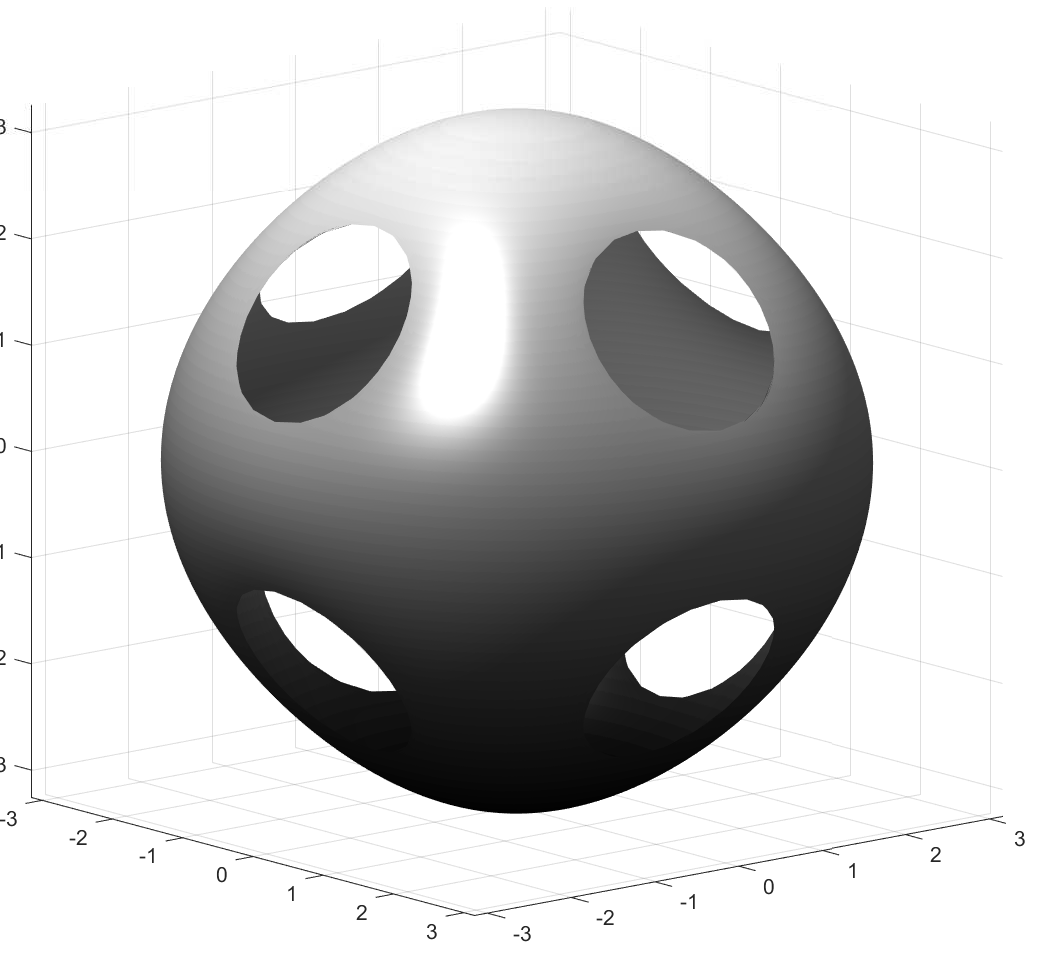
\includegraphics[width = 0.5\linewidth]{figures/Singular/sing-ext-3v.pdf}} &
\subcaptionbox{Internal Singularity contribution by gimbal\label{fig:sing_int1}}{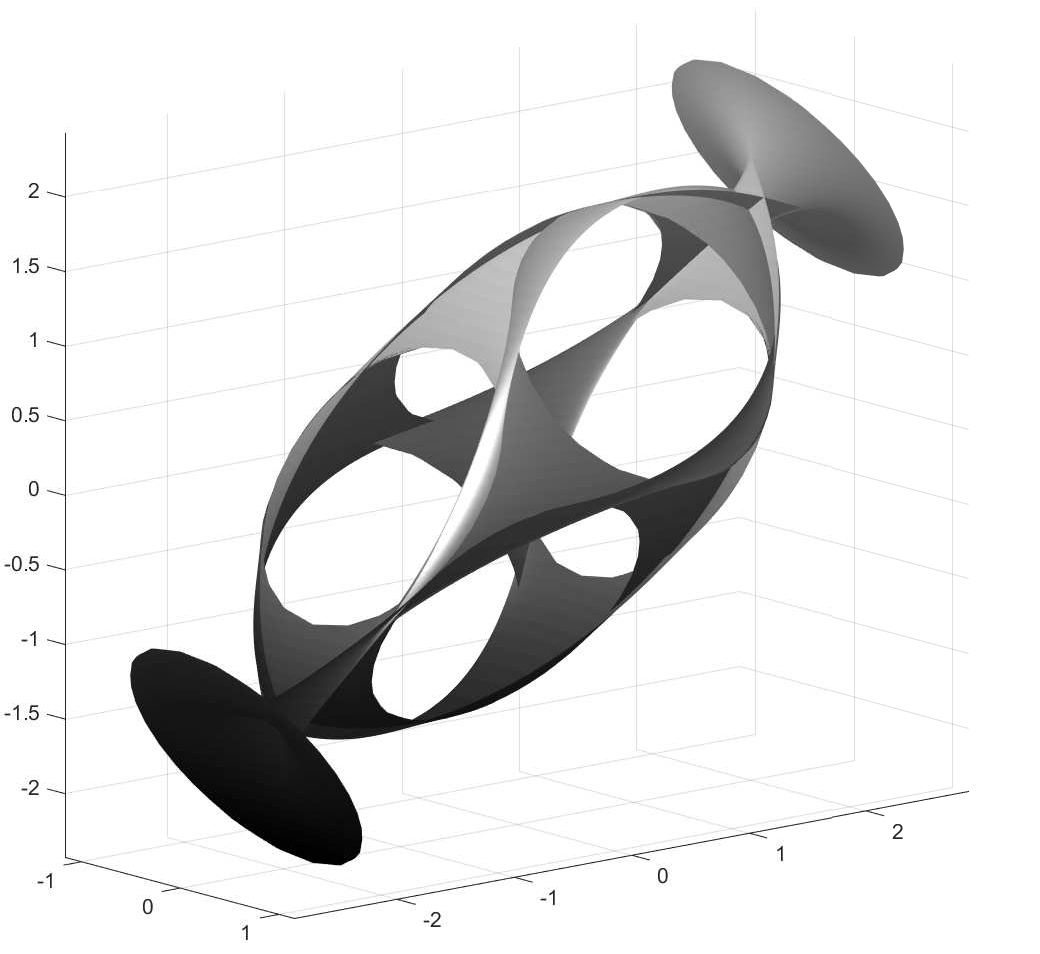
\includegraphics[width = 0.5\linewidth]{figures/Singular/sing-in-3v-1G.pdf}} \\

\subcaptionbox{Internal Singularity of all gimbals\label{fig:sing_int_all}}{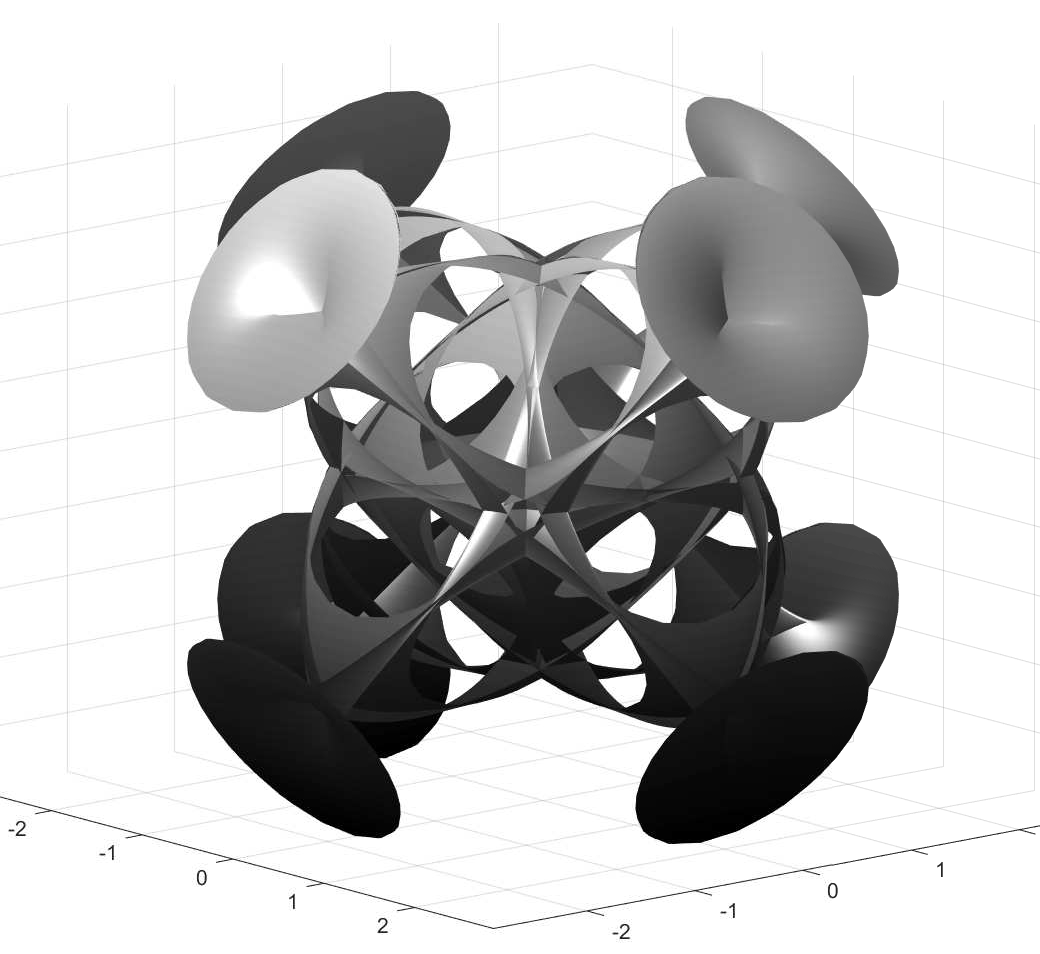
\includegraphics[width = 0.5\linewidth]{figures/Singular/sing-in-all3v.pdf}} &
\subcaptionbox{Singularities Combined\label{fig:sing_allOpq}}{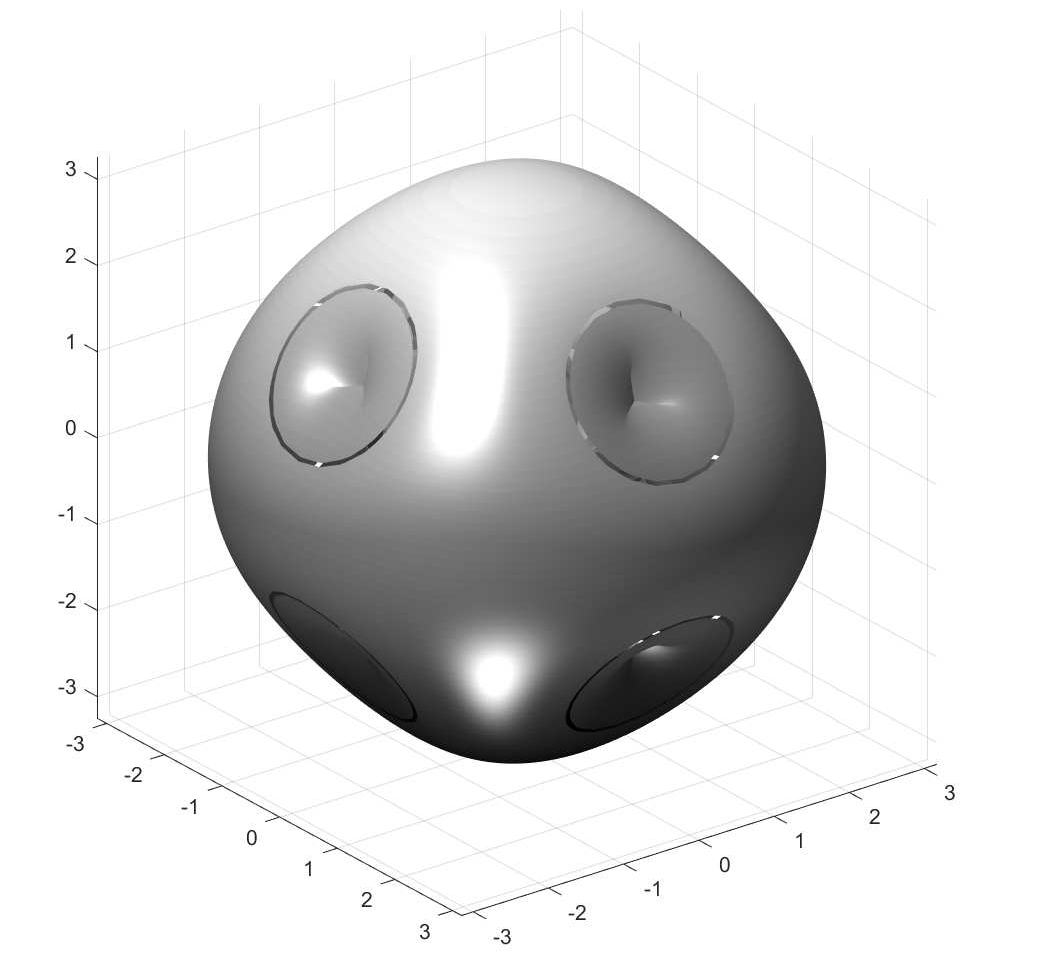
\includegraphics[width = 0.5\linewidth]{figures/Singular/sing-in-all3vOpeque.pdf}} \\
\multicolumn{2}{c}{\subcaptionbox{Singularities Combined\label{fig:sing_allTransp}}{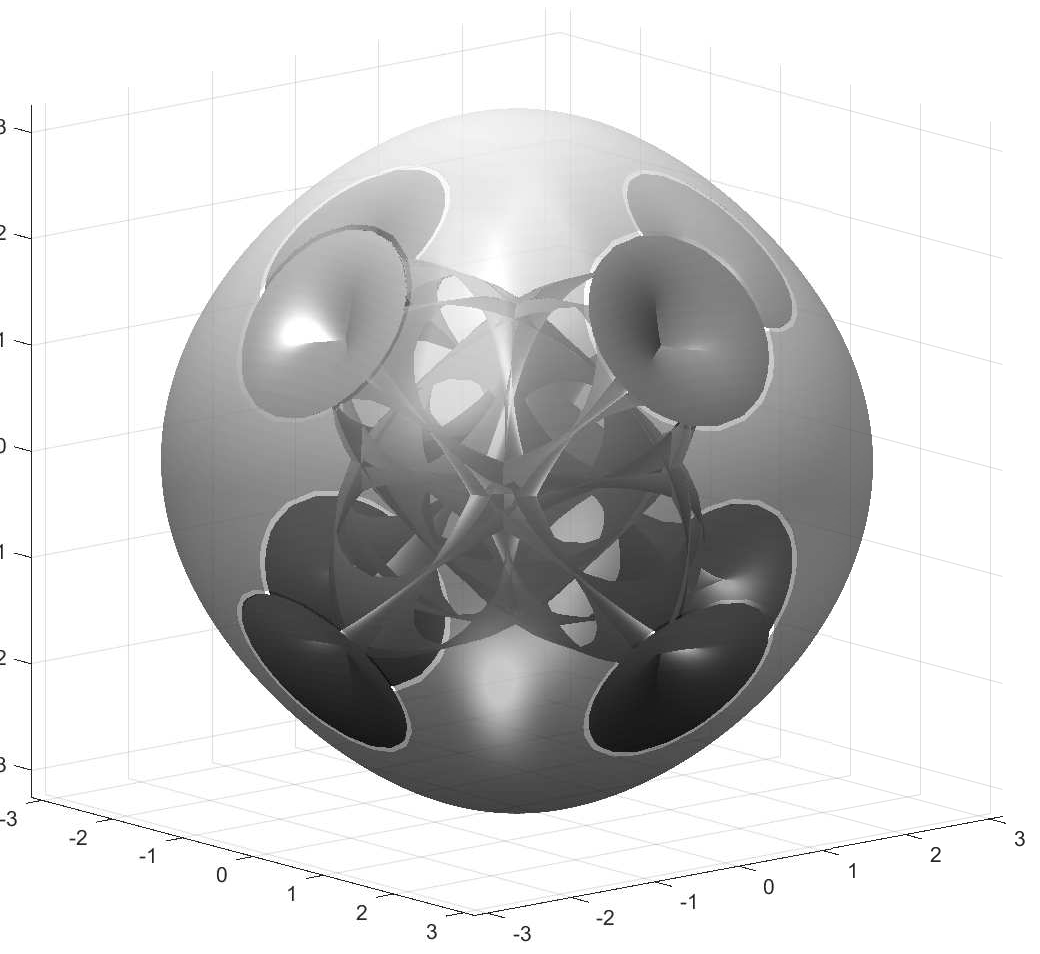
\includegraphics[width = 0.7\linewidth]{figures/Singular/sing-all-transperent.pdf}}}


\end{tabular}
\caption{Singular surface of control moment gyro in pyramid configuration with skew angle $\beta=54.73^\circ$}
\label{fig:singular_surf}
\end{figure}

